\documentclass[conference,letterpaper,11pt]{IEEEtran}
%\documentclass[conference,letterpaper]{IEEEtran}

\usepackage[english]{babel}
\usepackage[utf8]{inputenc}
\usepackage{amsmath}
\usepackage{graphicx}
\usepackage{fixltx2e}
\usepackage{array}

\title{Brisera: Distributed Read Mapping with Spark}

\author{
\IEEEauthorblockN{Benjamin~Bengfort}
\IEEEauthorblockA{University~of~Maryland\\ 
bengfort@cs.umd.edu}
}
% Your document starts here!
\begin{document}

% Define document title and author
	
	\maketitle

% Write abstract here
\begin{abstract}
	Recent developments in DNA sequencing have created a wealth of genomic data available for many different species to biologists.  It is no longer the case that single genomes are evaluated independently with a set of matching reads and the scale of the data continues to increase at a rapid pace. Simultaneously, recent developments in distributed computing techniques have created new opportunities for large scale cluster computing across thousands of nodes, particularly due to the open source framework \textit{Hadoop}. One of the first developments of parallel bioinformatics computing was \textit{BlastReduce} (now \textit{CloudBurst}) leveraged the MapReduce framework to improve multiple read alignments using the \textit{BLAST} algorithm. Hadoop is now mature as it enters its second decade, and has generalized cluster computing in such a way that new cluster computing paradigms are increasing in popularity, particularly \textit{Spark} - a generalized distributed computing framework that utilizes Resilient Distributed Data sets to effectively compute in-memory across nodes, elimination much of Hadoop's overhead. In this paper I will present an implementation of CloudBurst in Spark called Brisera that will be shown to perform more efficiently than Hadoop-based algorithms. 
\end{abstract}


\section{Introduction}
	Computational Biologists have benefited in rapid developments in genome sequencing over the past decade, and have come under a deluge of genomic data. Traditionally, single processor sequence alignment and matching algorithms were developed to be efficient in both time and space because of the length of a single genome. Because of developments in sequencing technology, it is no longer the case that genetic sequences are evaluated independently or singly. Data sets from new types of sequencing machines are comprised of millions of short sequences around 300bp of DNA called reads that are collected randomly from a DNA sample and must be assembled together \cite{bankier_shotgun_2001}. Importantly, these reads can also be aligned (mapped) to a reference genome to find the locations where the reads occur with some error threshold (in terms of the number of differences). This technique has many practical applications including comparing small differences in sequences between members of the same species, or to compare the evolved traits of different species, and are only possible due to the large number of sequences from multiple individuals available to researchers.
    
    In order to deal with the deluge of genomic data, there has been some work investigating the application of big data techniques researched in the distributed systems domain for application to bioinformatics problems \cite{taylor_overview_2010}. Highly available, large scale data stores like NoSQL databases make it efficient and easy to preprocess, index, and store kmers for fast lookups on reference material \cite{menon_rapid_2011,qiu_cloud_2009}. However, in order to effectively process hundreds of thousands of reads against reference sequences that are millions of bp long, a distributed computational framework is required. Hadoop \cite{dean_mapreduce_2008} is a mature, open source framework for distributed computation and data storage across thousands of nodes that provides a computational framework called MapReduce to parallelize algorithms, and is well researched for Bioinformatics applications \cite{leo_biodoop_2009,niemenmaa_hadoop_bam_2012,li_hadoop_2012}. 
    
    Of special interest to this paper is BlastReduce \cite{schatz_blastreduce_2008} (now updated to CloudBurst \cite{schatz_cloudburst_2009} which implemented the BLAST \cite{altschul_basic_1990} algorithm in a parallel fashion with MapReduce. BlastReduce is a seed and extend alignment algorithm optimized for mapping reads from next generation sequencing to larger reference genomes while allowing some differences. BlastReduce was shown to greatly improve performance over a single processor implementation of Blast. 
    
    Hadoop is quickly becoming adapted to a new general cluster computation engine, Spark \cite{zaharia_spark_2010} that promises to be more efficient by using in-memory computing for faster iterative algorithms and more friendly to develop. In particular, Spark allows for \textit{interactive} analysis of extremely large data sets, which can change the way that computational biologists explore and interact with large sequences. In this project I have explored the implementation of BlastReduce with Spark for read mapping short query sequences against larger reference genomes. I believe that Spark will perform better at scale than Hadoop, but I also discovered that the Spark implementation was simpler and more easily adaptable to different mapping applications.
    
\subsection{Spark}    
    
   	Although Hadoop is an well known open source framework, it does suffer from some performance limitations. First, the MapReduce API is limiting (developers are only given the option of Map and Reduce). In order to perform complex algorithms with Hadoop, data flows must be developed that chain MapReduce jobs together towards a final result. Moreover, between every MapReduce job, Hadoop is forced to serialize data to disk, incurring a significant IO penalty. Hadoop's framework was well suited to provide a shift in paradigm from message-passing distributed computations to more generally accessible ones, and eventually an Ecosystem developed with \textit{specialized} components for performing SQL-like operations on distributed data stores, working with higher order data flow tools, and to implement machine learning and graph algorithms that are difficult to express as MapReduce. However, all of these specialized tools had to be compiled to MapReduce in the end. 
    
    Spark introduces Resilient Distributed Data sets \cite{zaharia_resilient_2012} - an in-memory, fault-tolerant, partitioned object store that changed the way distributed computing could be implemented. RDDs provide the basic building blocks and invariants necessary for multiple nodes performing work on the data set via partitions, but because the application developer merely interacts with a list abstraction far more API functions are available than Map and Reduce. RDDs lay the ground work for a truly general cluster computing framework, and in fact Spark has Graph and Machine Learning libraries, a SQL-library, and a Streaming library already packaged as general dependencies. Graph and ML algorithms especially benefit from RDDs because the RDD is stored in memory, allowing for much faster iterative analysis, which most Graph and ML algorithms rely upon. Finally  Spark's API is developer friendly, available in three languages: Scala, Java, and Python - making it an excellent tool for computational biologists. 

\subsection{BlastReduce}

	BlastReduce is a parallel seed and extend algorithm implemented with MapReduce. BlastReduce uses fixed length mers as seeds to provide to the Landau-Vishkin \cite{landau_introducing_1986} algorithm to extend exact seed matches between reads and a reference genome to find alignments with at most k-differences in parallel. BlastReduce is specially designed for short reads with a small number of differences, e.g. k=2 or k=3 for 25-50bp reads. However, BlastReduce scales linearly with the number of reads, making it effective at computing in parallel across huge numbers of read-reference comparisons. 
    
    BlastReduce is implemented as 3 MapReduce jobs. The first, MerReduce maps finds mers of length \textit{s} that are exactly matched between the reads and the reference genome. To do this, for each mer in the input sequence (which includes both the reads and the reference) it maps all the seeds along with metadata and then reduces seeds that appear in both data sets. The second job, SeedReduce attempts to merge consistent shared mers into larger seeds (if they are within a threshold bp offset in the read and reference). This step, however, has been removed from the CloudBurst implementation. The last MapReduce job extends the seeds to find inexact alignments with only k-differences. For each shared seed from the MerReduce job, the mapper extends the seed using left and right flanks then aligns them with the discovered reference chunks via Landau-Vishkin. The reduce phase of ExtendReduce filters duplicate alignments and sorts the alignments in a sensible manner. 
    
    BlastReduce shows promising empirical results in terms of the running time of the algorithm compared to BLAST over millions of reads. BlastReduce uses some optimizations, for example Hadoop's SequenceFormat, which allows BlastReduce to serialize the sequence as a binary string and make very fast comparisons. However, as BlastReduce is implemented as three distinct MapReduce jobs, the output of each job (and the input to the next) must be written to disk first, then read from disk on the start of the next job. This happens twice in BlastReduce and causes considerable IO penalty, especially as the number of reads increases. 

	A final consideration of BlastReduce's implementation is that seeds from both the reads as well as the reference data sets must be processed together. In order to collect the two data sets for comparison, markers need to be stored along with the data in order to determine the differences between reference and read seeds at different phases in the processing. Although sequences are read in order (reads first with the reference following), the sequential, streaming read process of Hadoop requires BlastReduce to track the seeds throughout the algorithm. This is both inefficient in terms of processing as well as a significant challenge to developers trying to adapt BlastReduce to novel applications.

\section{Implementation}

	Brisera (in Swedish, burst or explosion), is an implementation of BlastReduce using Spark and RDDs rather than MapReduce. Brisera is implemented in Python and utilizes PySpark to run on a small cluster of machines in a parallel fashion. Like BlastReduce, Brisera also uses the Landau-Viskin algorithm for alignments and relies on very few external dependencies, and no bioinformatics dependencies like biopython. The code base is lightweight, especially when compared to BlastReduce as much of the cluster management overhead code and resource allocation is handled by Spark rather than by the developer. 
    
    Brisera uses a series of \textit{transformations} on multiple RDDs in order to perform its computation. Transformations are lazily evaluated by Spark - meaning that many transformations can be applied to a single RDD before execution takes place across the cluster. Such execution is usually initiated by an \textit{action} such as an aggregation or a required computation like join. Spark applications are composed of the creation of RDDs by reading data from disk, the transformation of RDDs through operations like filters, joins, or maps, and the execution of actions such as count or save to disk. While operations on RDDs are being carried out, the data is stored in memory on the nodes of the cluster; therefore as multiple transformation-action sequences are applied the system responds extremely quickly. 
    
    Using the ability to hold multiple RDDs in memory at a time, Brisera only used two transformation-action sequences unlike BlastReduce's three MapReduce jobs. First it created two RDDs for both the reads and reference data, then applied the seed reduction on each in parallel. The two RDDs were then joined by seed, and filtered such that they composed a single RDD of matching read, reference chunk pairs, that could then be aligned using dynamic programming sequence alignment. The sequence alignments were the most resource intensive operations of the entire process, and in fact the computation is limited by the number of allowed differences in the alignment (k). Once the alignments were returned, the final RDD was filtered and sorted such that only the best alignments remained, in the order of the reference genome. 

\section{Discussion}

	In order to compare CloudBurst to Brisera, I used a small sample data set containing 100,000 Illumina reads of length 36bp and a reference sequence from the streptococcus suis genome of length 2007491bp, which was divided into 32 overlapping chunks for partitioning across the cluster. My primary test was to run the alignment algorithm with varying k on 8 cores to see how the distributed algorithm would perform, especially related to the computational requirements for the dynamic programming alignments. 

	\begin{figure}[!hbt]
		% Center the figure.
		\begin{center}
		% Include the eps file, scale it such that it's width equals the column width. You can also put width=8cm for example...
		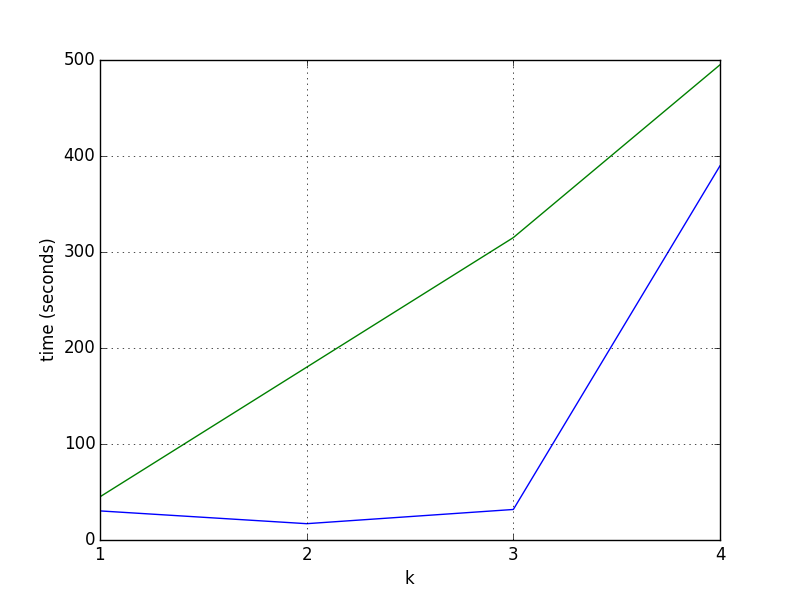
\includegraphics[width=\columnwidth]{figure_1}
		% Create a subtitle for the figure.
		\caption{Intermediate results: performance of CloudBurst vs Brisera on a small genome with varying k for 100,000 reads and a large reference sequence.}
		% Define the label of the figure. It's good to use 'fig:title', so you know that the label belongs to a figure.
		\label{fig:k_compute}
		\end{center}
	\end{figure}

	The Hadoop implementation of CloudBurst took approximately three minutes at k=3 to compute the alignments. The Spark implementation of Brisera took less than a minute (around 30-40 seconds) to compute the same alignments. This difference in time is wholly due to the fact that data resides in memory and is not written to disk between tasks in the algorithm. I experimented with different values of K to discover the base resource cost of Brisera, shown in \ref{k_compute}. The performance cost of CloudBurst is linear with the number of reads as well as the value of k. Brisera's performance is also proportional to the number of reads, but it only incurs this cost once. For both CloudBurst and Brisera, the effect of higher k values can be minimized by adding more nodes with higher available memory, but the cost in terms of time will always be related to the computational expense of the dynamic programming alignment. 
    
    Unfortunately due to travel and budget constraints (the cluster I was using to compute on was made unavailable) I was unable to perform a large scale test - namely the performance in terms of time vs. the number of reads for both Coudburst and Brisera on a small cluster of 20-30 nodes. Using Amazon EC2's cloud, I estimate that the cost of such an experiment would be \$40-\$80, and I hope that someone is willing to spend this amount of money to further explore Spark for bioinformatic applications in the future! 


\section{Conclusion}
	
    In this short paper I have presented Brisera, an implementation of BlastReduce using Spark's general cluster computation engine instead of MapReduce. Brisera was lightweight and extremely easy to implement, especially compared to the much heavier Java code that is required to implement MapReduce jobs. Brisera was implemented in Python and had far fewer developer challenges due to the fact that it was unnecessary to conform to the rigid MapReduce structure. Instead of mingling reads and reference chunks, Brisera kept them in separate distributed data structures, operating on them independently in a parallel fashion until they could be aligned together. Moreover, because Spark keeps data structures in memory on nodes rather than incurring disk IO costs, it was significantly faster to perform the alignment than using Hadoop. 
    
    Because Spark is a general computation framework that provides many transformations and actions on an sequence of distributed objects (an excellent storage structure for genetic sequences) it will become an increasingly important tool for computational biologists in the future, especially as DNA sequencing technology becomes cheaper. Not only is Spark friendly to developers, but it also has interactive analysis and very fast iterative optimization algorithms that will be essential to exploring sequences and alignments in the future. 
    
\bibliographystyle{plain}
\bibliography{references}

% Your document ends here!
\end{document}